See 
		\figref{fig:11/10/2/10}.
	\begin{figure}[H]
		\centering
 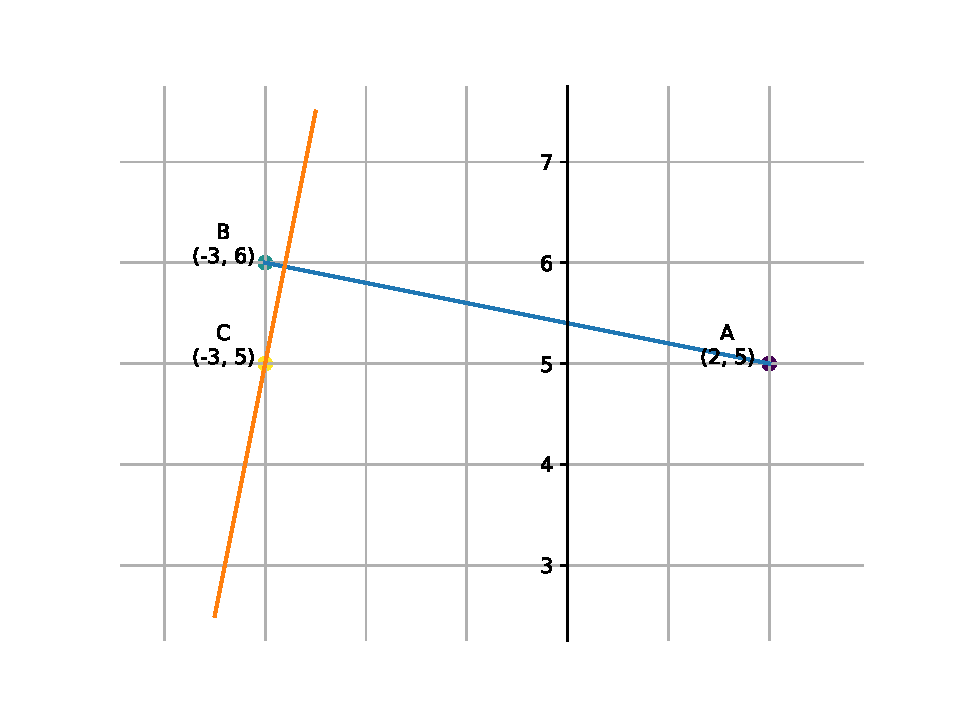
\includegraphics[width=0.75\columnwidth]{chapters/11/10/2/10/figs/fig.pdf}
		\caption{}
		\label{fig:11/10/2/10}
  	\end{figure}
The normal vector is
\begin{align}
\vec{n} =\myvec{2 \\5} -  \myvec{-3 \\ 6} 
=\myvec{
    5\\
    -1
}
\end{align}
Thus, the equation of the line is 
\begin{align}
\myvec{
    5 &-1
	}\brak{\vec{x} - \myvec{-3 \\5}}
= 0
\\
\implies 
\myvec{
    5 &-1
	}\vec{x} 
= -20
\end{align}
